\section{The Peer-to-Peer Network Architecture}
In the peer-to-peer network architecture, every node in the system
contributes with its resources, including both storage space and
processing power.

Popularised through file sharing, found its way into academia, dhts,
distributed systems

\section{The Publish-Subscribe Communication Paradigm}

Publish-Subscribe is a fully asynchronous, loosely coupled,
highly scalable, event-based messaging pattern. There are three main
system components in the pub/sub interaction scheme: the publishers, the
subscribers and the event service. The publishers publish events, and
the subscribers subscribe for events, while the event service handles
managing both subscriptions and publications, as well as routing events
to the subscribers. The basic architecture of a typical pub/sub system
is outlined in Figure~\ref{fig:pubsubarch}.

\begin{figure}
\centering
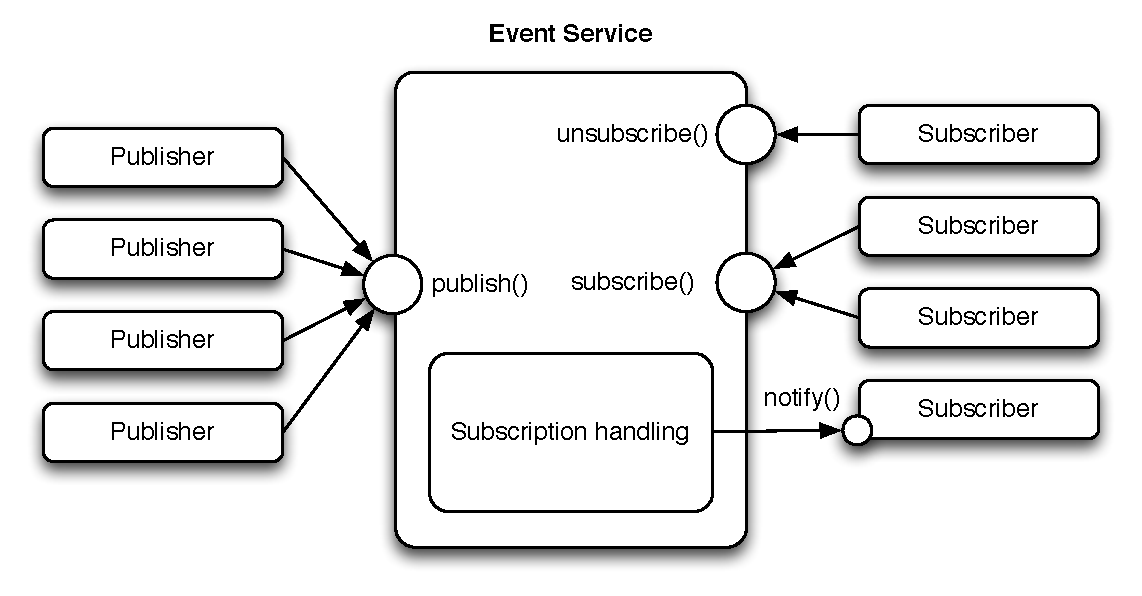
\includegraphics[width=\textwidth]{figures/pubsubarch}
\caption{The basic architecture of a pub/sub system.}
\label{fig:pubsubarch}
\end{figure}

The event service functions as an intermediary between publishers and
subscribers. It provides a level of indirection, as well as an service
interface. Publishers are able to generate new events through the
\texttt{publish} service call. It is now the responsibility of the event
service to determine which subscribers are interested in receiving this
event, and how to route the event to them. The subscribers register
their interest through a \texttt{subscribe} service call. The event
service will then store each subscribers interest in order to
disseminate events correctly. The publishers are then able to cancel
their subscriptions through a \texttt{unsubscribe} service call. No
information is forwarded from subscribers to publishers or from
publishers to subscribers.

The pub/sub paradigm provides a higher degree of decoupling than other
traditional approaches. In general there are three types of decoupling
pub/sub system provides us with:

\begin{description}
  \item[Space decoupling] The publishers and subscribers does not need to
    know about each other.
  \item[Time decoupling] Events are delivered regardless of whether or
    not publishers and subscribers are online at the same time.
  \item[Synchronization decoupling] Neither publishers nor subscribers
    are blocked when attempting to perform their operations.
\end{description}

While many other approaches can provide the first two forms of
decoupling, the main advantage of pub/sub is its fully asynchronous nature.
Approaches such as tuple spaces or message queues cannot completely
provide this synchronous decoupling, as messages are retrieved in a
synchronous manner. This property is key to the suitability for pub/sub
in large distributed system.~\cite{Eugster:2003}

\subsection{Message Filtering in Pub/Sub}

The subscription semantics of the pub/sub paradigm plays an important
role in the performance and flexibility of the system as event messages
are routed and managed based on topic or content. There are three
distinct types of subscription schemes:

\begin{description}
  \item[Topic-based] Events are split into topics, usually represented by
      a string.
  \item[Type-based] Filters events based on the structure of the data.
      Provides type safety at compile time.
  \item[Content-based] Events are filtered based on a global
      list of universal event attributes.
\end{description}

Content-based provides better expressiveness in terms of filtering out
the relevant events. However, this comes at the cost of higher overhead
with regards to handling subscriptions. The complex filtering algorithms
limit the scalability of such systems with regards to the number of
subscriptions. Type based is similar to content-based in the sense that
the public members of the types together form a description of the
content of the event. Although this ties the implementation of the
pub/sub system closer to the programming language, it still suffers from
the same drawbacks as content-based.

Topic-based offer less expressiveness than the other two subscription
schemes, but better performance if the set of possible event properties
is limited. Also, topic-based is more suited for dissemination and
multicasting, as topics can be thought of as groups, where subscribing
to topic T can be equivalent to joining the group for that topic. This
is the approach taken by several proposed pub/sub systems which will be
discussed later in this paper.

Traditionally, reliable multicasting of data through deterministic
dissemination has been the common approach. However, more recent
implementations investigate the potentials of probabilistic protocols,
which are more suited to the nature of decentralized systems and P2P.
These protocols do not guarantee full reliability, but provides a high
quantifiable \emph{probability} that events are delivered to all
subscribers.

\section{Online Social Networks}
What is an OSN?\ Impact on networks?\ What approaches?\ Decentralised OSNs?
\section{Social Network Analysis}
What is SNA?\ What are the common characteristics of a Social Graph?\
Actors, How to measure influence/power of actors (centrality?)
\section{Dynamic Network Analysis}
emerging field.
\section{Pub/Sub in Online Social Networks}
Is Pub/Sub being used in social networks?\, In Spotify? (nudge nude, wink wink) Why is it
useful?\
